\chapter{Human Visual System}%
\label{ch:hvs}

To produce colour images of a scene on a digital camera that resembles how a human might perceive it, it is important to understand how the human visual system functions. A cross-section of the human eye is shown in \ref{fig:humaneye}. Many parts of the human eye have direct correspondences in a typical digital camera, such as the lens (and cornea) which focuses an inverted image onto the retina, similar to how a lens in a digital camera focuses the image to a sensor. The ciliary muscles attached to the lens can also change its shape, when focusing at different distances is required, much like how camera lenses with variable focal length work. The pupil and iris together create a system that is comparable to the adjustable aperture of a digital camera, controlling the amount of light that enters the eye.

\begin{figure}
    \centering
    \pdftooltip{
\includegraphics[width=0.7\textwidth]{figures/eye.eps}}{lol}
    \caption{Cross-section of the human eye \cite{humaneye}}
    \label{fig:humaneye}
\end{figure}

\section{Retinal receptors}

At its core, the retina of the human eye consists of receptors of different, which can be divided into two subtypes, rods and cones. The former operates primarily during dim light conditions, when the human vision is said to be scotopic, while the latter operates during well lit conditions.


The rods activate during low-light conditions, such as under moonlight, providing us monochromatic "night vision", more commonly referred to as the scotopic vision. On the contrary, the cones operate during well-lit conditions, such as daylight, allowing us to perceive colours while the photopic vision system is active. The reason why colours are perceivable during photopic vision and not scotopic vision is, that there are three types of cones, each sensitive to different range of visible wavelengths, while there is only one a single cone type.  \cite[4-5]{measuringcolour}

On the boundaries of these two conditions, known as the mesopic vision, both the rods and cones are active, which results in a phenomenon where colours are visible but they appear darker and blue-ish. This is known as the Purkinje effect. \cite[5]{measuringcolour}

\section{Spectral responsivity}

% Although Newton, using a prism, had already discovered in the 17th century that white light is a combination of several color components of different wavelengths, it was not until centuries later, that the trichromatic theory was proposed by Young. The theory suggested that the human eye consists of three receptors, sensitive to red, green and blue wavelengths respectively, and all colours could be produced by a mixture of them. Experiments during the 20th century have proven this to be partially correct, as there are three types of color receptors that form the primary response to those exact colours, but they also respond to larger range of colors. \cite{colorimetry}

% Various other theories were also proposed in addition to the trichromatic theory, such as the opponent-color theory, and produced results that were supported by empiric results and could explain certain phenomena \cite{colorimetry}. Robust test scenarios were designed during the 20th century to measure the relative responsiveness of cones and rods. By evaluating the relative responses at a densely sampled interval, spectral responsivity curves are obtained. \cite{measuringcolour} Readers interested in details of these measurements can be referred to chapters 1 and 2 in \cite{measuringcolour} and chapters 1-3 in \cite{colorimetry}.

To be able to model the human eye computationally, such as in digital cameras, its important to quantify how sensitive the eye is at some wavelength relative to some other wavelength. A standard was published in 1931 consisting of data collected by Wright and Guild from psychovisual experiments on subjects with standard vision under photopic vision. The subjects were asked to match a reference light, at some known wavelength, using a combination of three different lights with wavelengths of 435.8, 546.1 and 700 nm, corresponding roughly to the blue, green and red wavelengths respectively. \cite{wrightetguild}

These results from the two observers were combined and standardized by CIE (Commission internationale de l'éclairage), an international commission on illumination \cite{CIE}. The so called CIE 1931 RGB color matching functions are shown in figure \ref{fig:rgb}, which denote the amount of each color to match the reference light. The choice of three primaries posed some problems, as its not possible to match every color with three primaries, and thus for example red is negative in the range of 450-550 nm, as some of it had to be added to the reference light instead of the to the combination of two other primaries. \cite{measuringcolour}

To simplify computations and to make the model more interpretative, at the same time in 1931 introduced another set of color matching functions based on the previous, but with an idea that all the functions should be strictly positive, and one of them should correspond to the luminance of the color. Thus another, much more widely used, set of functions called the CIE 1931 XYZ color matching functions, was published. The functions are shown in figure \ref{fig:xyz}.


%The entity responsible for standardizing the results of these measurements is CIE (Commission internationale de l'éclairage) \cite{CIE}. They have released several standardized spectral responsivity curves, such as the spectral luminous efficiency function under scotopic vision for the standard observer in 1924, and similary for photopic vision in 1955 \cite{observer}. These measure the relative brightness across the visible wavelength range, and have been computed as the average of multiple observers with normal vision.

%In 1931, CIE published perhaps its most important standard for the colour industry, namely the 1931 CIE colour matching functions (CMFs), based on measurements by Wright and Guild. These define the relative amounts of the three colour primaries Red (700 nm), Green (546.1 nm) and Blue (435.8 nm) that are required to reproduce every colour in the visible range.\cite{measuringcolour} The function is seen in figure \ref{fig:rgb}.

\begin{figure}
    \centering
    \pdftooltip{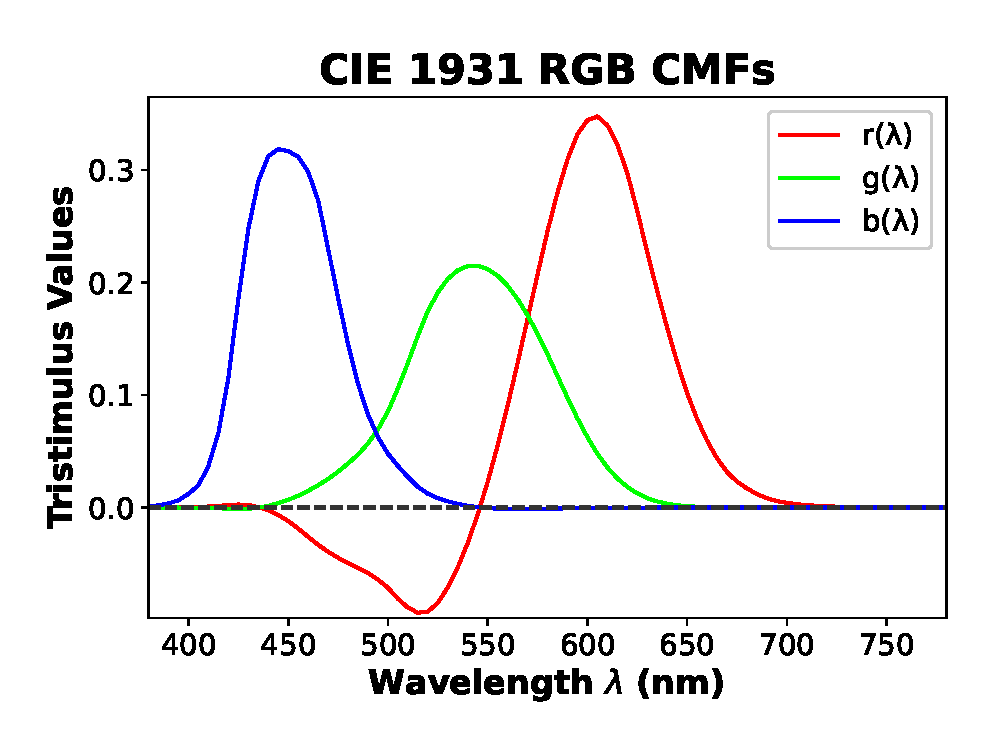
\includegraphics[width=\textwidth]{figures/cie_rgb.eps}}{CIE RGB CMFs}
    \caption{CIE RGB  \cite{humaneye}}
    \label{fig:rgb}
\end{figure}

\begin{figure}
    \centering
    \pdftooltip{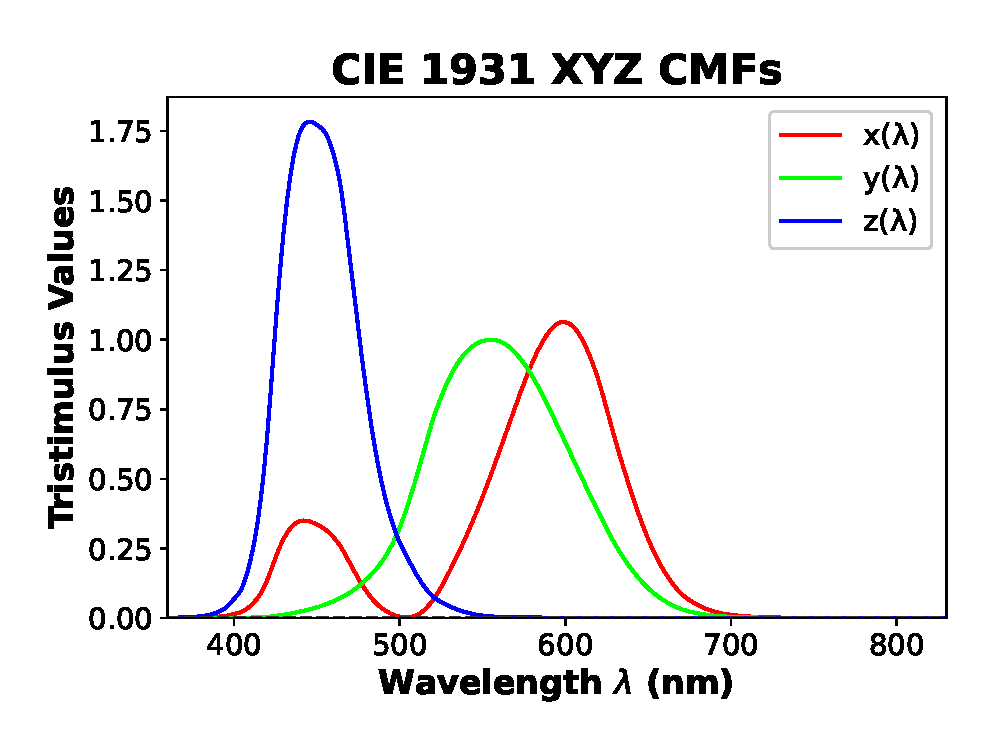
\includegraphics[width=\textwidth]{figures/cie_xyz.eps}}{CIE XYZ CMFs}
    \caption{CIE XYZ  \cite{humaneye}}
    \label{fig:xyz}
\end{figure}

\section{Tristimulus values}

From the spectral sensitivities shown in figures \ref{fig:rgb} and \ref{fig:xyz}, its possible to compute the so called tristimulus values, which mathematically describe the response of the eye to to the light that reaches the retina. The responses are computed by integrating the product of the illuminant's power spectral distribution, spectral reflectance of the object and the spectral responsivity of the sensor for given colour.

As one of the components, Y, corresponds to the luminance of the color, it makes sense to normalize it between 0 and 100 to treat is a percentage. The normalization factor $k$ can be computed as the response of the Y channel to light reflected from a perfectly white surface with Lambertian reflectance as follows

\begin{equation}
\label{eq:normalization}
 k = \frac{100}{\int_{380}^{780} E(\lambda) S_Y(\lambda) \, d\lambda},
\end{equation}

where $100$ is a scaling factor, $E(\lambda)$ is the spectral power distribution of a given illuminant, and $S_Y(\lambda)$ is the cone sensitivity for Y \cite{rowlands2020physics}. Note, that $1$ is often used as the scaling factor in numerical computation for simplicity.

The tristimulus value $T$ corresponding to either $X$, $Y$ or $Z$ is then given by

\begin{equation}
\label{eq:tristimulus}
T = k \int_{380}^{780} E(\lambda) R(\lambda) S_T(\lambda) \, d\lambda,
\end{equation}

where $E(\lambda)$ is the spectral power distribution (SPD) of the illuminant, $R(\lambda)$ is the spectral reflectance of the object, and $S_T(\lambda)$ is the sensitivity of the cones for tristimulus value \( T \) (either \( X, Y, \) or \( Z \)).

\begin{figure}
\centering
\scalebox{1.5}{%
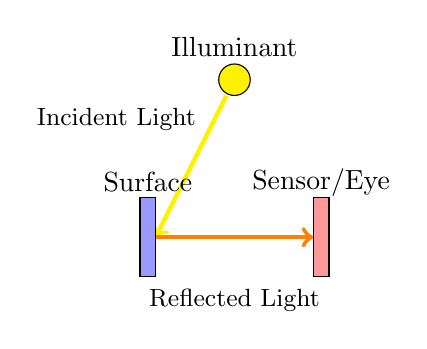
\begin{tikzpicture}
  
  % Set the bounding box manually for more space at the bottom

  % Illuminant
  \draw[fill=yellow] (2,3) circle [radius=0.2] node[above=5pt] {Illuminant};
  \draw[->, ultra thick, yellow] (1.9,2.8) -- (1,1);

  % Surface
  \draw[fill=blue!40] (0.8,1.5) rectangle (1,0.5) node[midway, yshift=0.7cm] {Surface};

  % Sensor/Eye
  \draw[fill=red!40] (3,1.5) rectangle (3.2,0.5) node[midway, yshift=0.7cm] {Sensor/Eye};
  \draw[->, ultra thick, orange] (1,1) -- (3,1);

  % Annotations without lines
  \node[font=\small] at (0.5,2.5) {Incident Light};
  \node[font=\small] at (2,0.2) {Reflected Light};

\end{tikzpicture}
}


\caption{Light to eye model}
\label{fig:light}
\end{figure}

\section{Chromatic Adaptation}
\label{sec:chromaticadaptation}
Although one would assume that the tristimulus system is enough to model the human visual system, the human eye has the ability to adapt these sensitivities under different illuminant conditions. Even though the same scene under two different illuminants will produce distinct tristimulus values, the human visual system will perceive the colours the same. For example, a white sheet of paper will look white under sunlight and fluorescent light source. This feature is called chromatic adaptation. \cite[146-149]{fairchild}

Lots of research has addressed this phenomena during the past century, and the current ideas are only approximations of the complex biological process. The most common and oldest hypothesis was proposed by Johannes von Kries in 1902, where he suggested that the human visual system adapts to changing illumination by applying gain multipliers to the cone sensitivities. \cite[168-171]{fairchild} This effectively results in a set of coefficients for each illuminant, and can be mathematically formulated as follows

\begin{equation}
\begin{bmatrix}
L' \\
M' \\
S' \\
\end{bmatrix}
=
\begin{bmatrix}
1/k_L & 0 & 0 \\
0 & 1/k_M & 0 \\
0 & 0 & 1/k_S \\
\end{bmatrix}
\begin{bmatrix}
L \\
M \\
S \\
\end{bmatrix}
,
\end{equation}

where $L$, $M$, $S$ are the responses of the Long, Medium and Short wavelength cones to the original light source, $L'$, $M'$, $S'$ are the transformed responses after adaptation, and $k_L$, $k_M$, $k_S$ are the von Kries coefficients. The can be computed by substituting the Y channel sensitivity with cone sensitivities in formula \ref{eq:normalization}, using an appropriate scaling factor instead of $100$. This formula effectively removes effect of the illuminant and ensures that neutral objects have the same response under every light source.

Even in his publication, von Kries argued that his proposal was a gross oversimplification, but in practice, the method is still applied and it has been proved to be a good approximate \cite[170-171]{fairchild}. For example, consumer digital cameras often follow this model when simulating chromatic adaptation. More sophisticated models of chromatic adaptation exist, such as the Retinex Theory \cite{land1977retinex} or Bradford Transform \cite{lam1985metamerism}, but as we do not emphasize chromatic adaptation in this thesis, we only consider the von Kries transform in subsequent chapters for practical purposes.